\section{Analytical Model}
\label{sec:analytical-model}
In this Section we define the analytical model of the system.
%
In particular, we will first show the Markov Chain and flow balance equations for a very simple case, in order to introduce the reader to the structure of the chain with its critical states.
%
Then, we will show formulas for the performance metrics in the general case.
%
At the end, we will explain how we solved the analytical model to obtain theoretical results for the target case.

The analytical model is depicted in Figure~\ref{fig:analytical-model}, whose \textit{routing probabilities} are defined in Equation~\ref{eqn:routing-probabilities}.
The definition of routing probabilities relies on the following subsets of states $S_{clt,i} \subset S_{clt}$:

\begin{itemize}
	\item $S_{clt,1}$:  a task belonging to the $1^{st}$ class is accepted in the Cloudlet.
	
	\begin{equation}
	S_{clt,1} := \{(n_{clt,1},n_{clt,2})\in S_{clt} : n_{clt,1}+n_{clt,2}<N \vee n_{clt,2}>0\}
	\end{equation}
	
	\item $S_{clt,2}$: a task belonging to the $2^{nd}$ class is accepted in the Cloudlet.
	
	\begin{equation}
	S_{clt,2} := \{(n_{clt,1},n_{clt,2})\in S_{clt} : n_{clt,1}+n_{clt,2}<N \wedge n_{clt,2}<S\}
	\end{equation}
	
	\item $S_{clt,3}$: a task belonging to the $2^{nd}$ class is interrupted in the Cloudlet and it is restarted in the Cloud.
	
	\begin{equation}
	S_{clt,3} := \{(n_{clt,1},n_{clt,2})\in S_{clt} : n_{clt,1}+n_{clt,2}=N \wedge n_{clt,2}>0\}
	\end{equation}
\end{itemize}

\begin{figure}
	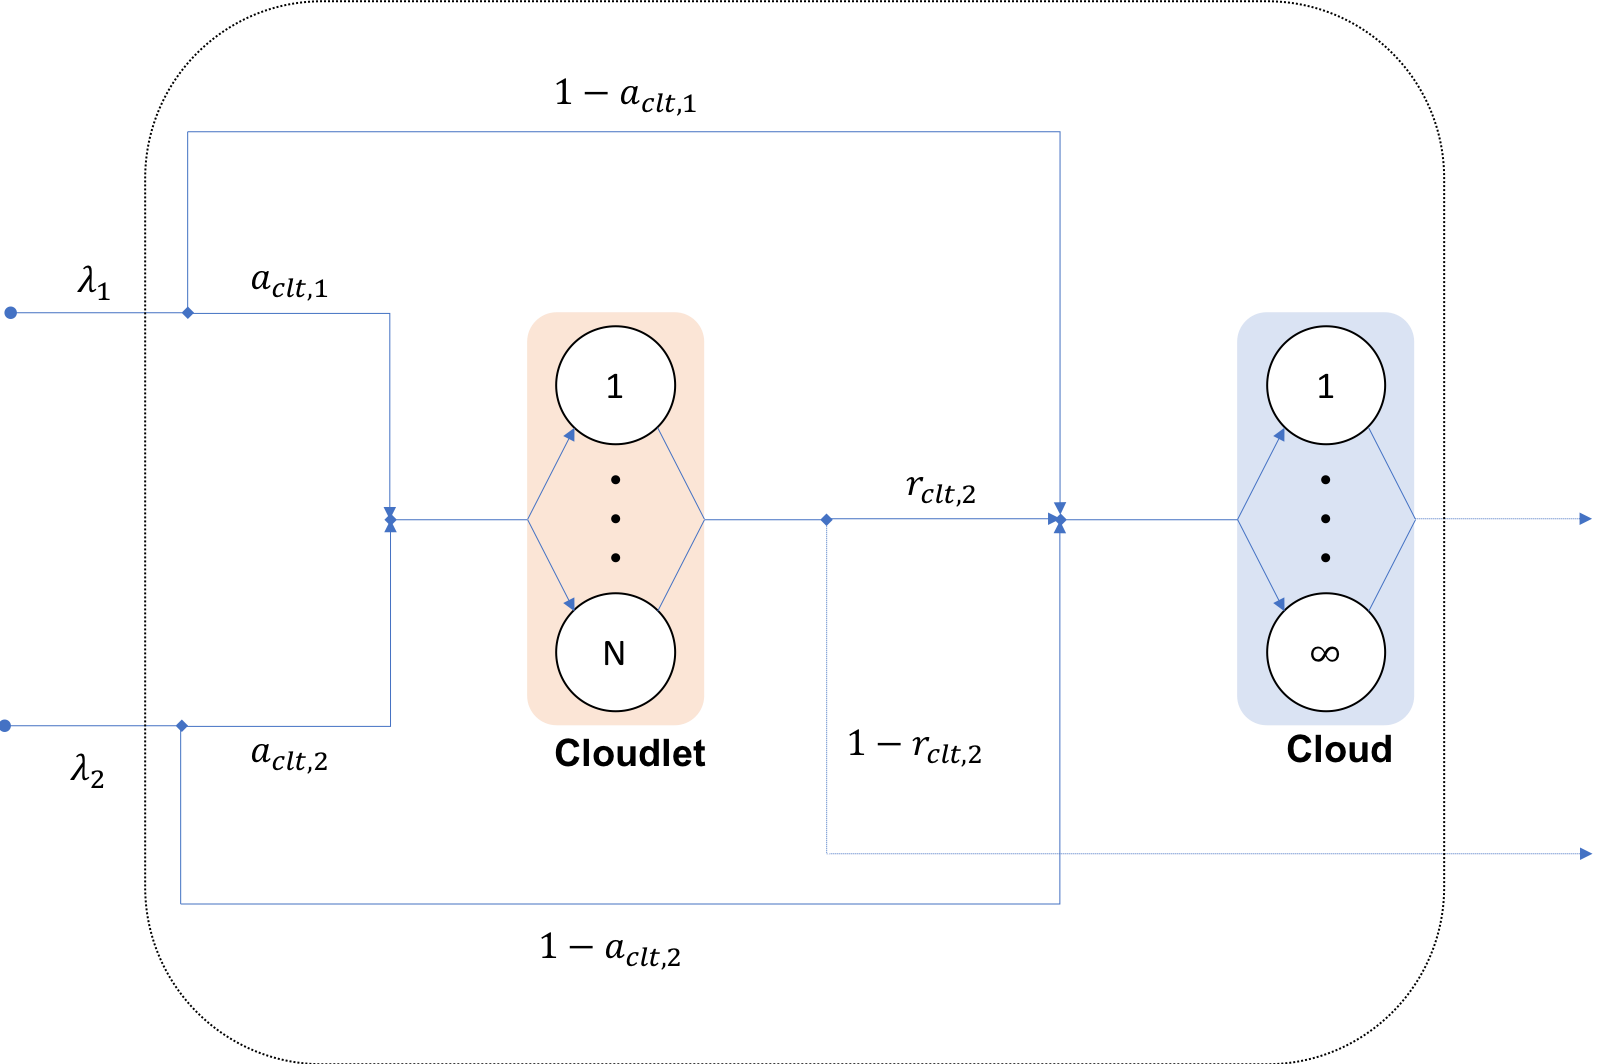
\includegraphics[width=\columnwidth]{fig/analytical-model}
	\caption{Analytical model.}
	\label{fig:analytical-model}
\end{figure}

\begin{equation} 
\begin{split}
a_{clt,1} & = \sum_{s\in S_{clt,1}} \pi_{s} \\
a_{clt,2} & = \sum_{s\in S_{clt,2}} \pi_{s} \\
r_{clt,2} & = \sum_{s\in S_{clt,3}} \pi_{s} \Big(\frac{\lambda_{2}}{\lambda_{1}+\lambda_{2}}\Big) \\
\end{split}
\label{eqn:routing-probabilities}
\end{equation}


\paragraph{Markov Chain}
As the Markovian condition holds true for our system, i.e. Poisson arrivals\footnote{same as Exponential inter-arrivals.} and Exponential services, we can determine the Markov Chain\footnote{If the Markovian condition is not satisfied, Markov Chain solution must be considered only an approximation.} whose resolution allows us to compute the routing probabilities shown in Equation~\ref{eqn:routing-probabilities}.

In Figure~\ref{eqn:analytical-model-markov} we show the Markov Chain with the associated flow balance equations listed in Equation~\ref{eqn:analytical-model-markov}.
For sake of simplicity, we consider here the simple case with $N=S=2$ in order to (i) give an idea of the system of equations to be solved and (ii) graphically recognize the critical states. In fact, the representation fo the Markov Chain and the associated equations would be inpractical for the case $N=S=20$, due to the combinatorial explosion of the state space.

In the considered simple case, the critical states are:

\begin{itemize}
	\item $(2,0)$: every arrival is forwarded to the Cloud;
	
	\item $(1,1)$: every arrival belonging to class 1 is accepted in Cloudlet, causing the restart in Cloud of the serving task belonging to class 2; whilst every arrival belonging to class 2 is forwarded to Cloud;
	
	\item $(0,2)$: every arrival belonging to class 1 is accepted in Cloudlet, causing the restart in Cloud of a random serving task of Class 2; whilst every arrival belonging to class 2 is forwarded to Cloud;
\end{itemize}

\begin{figure}
	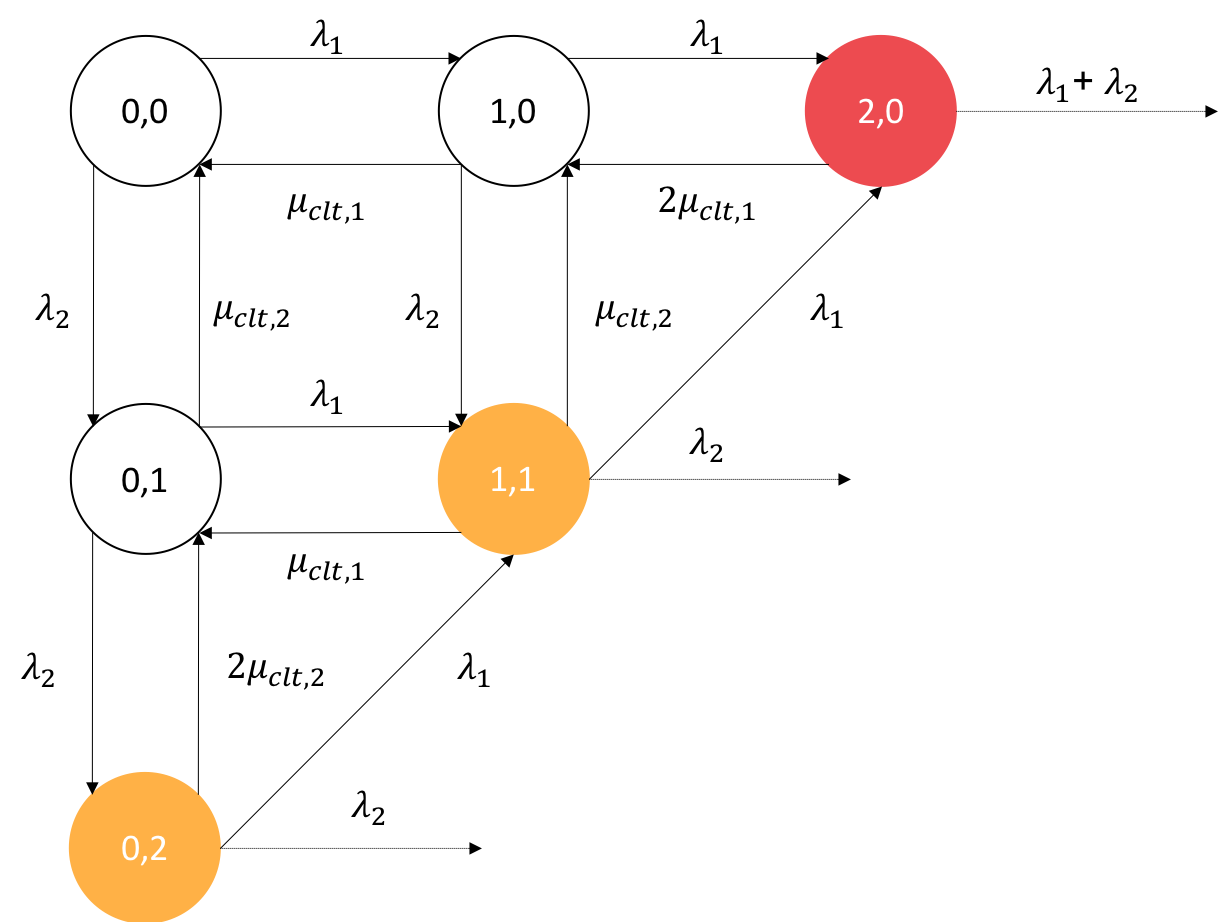
\includegraphics[width=\columnwidth]{fig/analytical-model-markov}
	\caption{Markov Chain with $N=2$ and $S=2$.}
	\label{fig:analytical-model-markov}
\end{figure}

\begin{equation} 
\begin{split}
\pi_{0,0}(\lambda_{1}+\lambda_{2})& = \pi_{1,0}\mu_{clt,1}+\pi_{0,1}\mu_{clt,2} \\
\pi_{0,1}(\lambda_{1}+\lambda_{2}+\mu_{clt,2}) & = \pi_{0,0}\lambda_{2}+\pi_{1,1}\mu_{clt,1}+\pi_{0,2}2\mu_{clt,2} \\
\pi_{1,0}(\lambda_{1}+\lambda_{2}+\mu_{clt,1}) & = \pi_{0,0}\lambda_{1}+\pi_{1,1}\mu_{clt,2}+\pi_{2,0}2\mu_{clt,1} \\
\pi_{1,1}(\lambda_{1}+\mu_{clt,1}+\mu_{clt,2}) & = \pi_{0,1}\lambda_{1}+\pi_{1,0}\lambda_{2}+\pi_{0,2}\lambda_{1} \\
\pi_{0,2}(\lambda_{1}+2\mu_{clt,2}) & = \pi_{0,1}\lambda_{2} \\
\pi_{2,0}2\mu_{clt,1} & = \pi_{1,0}\lambda_{1}+\pi_{1,1}\lambda_{1} \\
1 & = \pi_{0,0}+\pi_{0,1}+\pi_{1,0}+\pi_{1,1}+\pi_{0,2}+\pi_{2,0}\\
\end{split}
\label{eqn:analytical-model-markov}
\end{equation}

\paragraph{Accepted Workload}
Given the routing probabilities we can determine the following \textit{accepted workloads}:

\begin{itemize}
	\item \textit{Cloudlet}: arrival rate of tasks belonging to $j$-th class accepted in Cloudlet:
	\begin{equation}
	\lambda_{clt,j} = a_{clt,j}\lambda_{j}
	\end{equation}
	
	\item \textit{Cloud}: arrival rate of tasks belonging to $j$-th class forwarded to Cloud:
	\begin{equation}
	\lambda_{cld,j} = (1-a_{clt,j})\lambda_{j}
	\end{equation}
	
	\item \textit{Restarts}: rate of tasks belonging to $2^{nd}$ class interrupted in Cloudlet and restarted in Cloud:
	\begin{equation}
	\lambda_{r} = r(\lambda_{1}+\lambda_{2})
	\end{equation}
\end{itemize}

\paragraph{Performance metrics}
Given the accepted workloads we can determine the following \textit{performance metrics for classed tasks in each subsystem}.
%
We assume here to know the expected time lost in Cloudlet by $2^{nd}$ class tasks before their interruption. In particular, as we are not able to determine $E[T_{clt,2,lost}]$ from the Markov Chain, we will assume the experimental value computed by the simulator.

\begin{itemize}
	\item $1^{st}$ class in Cloudlet:
	\begin{equation} 
	\begin{split}
	E[T_{clt,1}] &= \frac{1}{\mu_{clt,1}} \\
	E[N_{clt,1}] &= \lambda_{clt,1}E[T_{clt,1}] \\
	\end{split}
	\end{equation}

	\item $2^{nd}$ class in Cloudlet:
	\begin{equation} 
	\begin{split}
	E[T_{clt,2}] &= \frac{1}{\mu_{clt,2}} \\
	E[N_{clt,2}] &= \lambda_{clt,2}E[T_{clt,2}]-\lambda_{r} E[T_{clt,2,lost}] \\
	\end{split}
	\end{equation}
	
	\item $1^{st}$ class in Cloud:
	\begin{equation} 
	\begin{split}
	E[T_{cld,1}] &= \frac{1}{\mu_{cld,1}} \\
	E[N_{cld,1}] &= \lambda_{cld,1}E[T_{cld,1}] \\
	\end{split}
	\end{equation}
	
	\item $2^{nd}$ class in Cloud (not restarted):
	\begin{equation} 
	\begin{split}
	E[T_{cld,2}]^{[NR]} &= \frac{1}{\mu_{cld,2}} \\
	E[N_{cld,2}]^{[NR]} &= \lambda_{cld,2}E[T_{cld,2}]^{[NR]} \\
	\end{split}
	\end{equation}
	
	\item $2^{nd}$ class in Cloud (restarted):
	\begin{equation} 
	\begin{split}
	E[T_{cld,2}]^{[R]} &= E[T_{setup}]+ E[T_{cld,2}]^{[NR]} \\
	E[N_{cld,2}]^{[R]} &= \lambda_{r}E[T_{cld,2}]^{[R]} \\
	\end{split}
	\end{equation}
	
	\item $2^{nd}$ class in Cloud (both restarted and not restarted):
	\begin{equation} 
	\begin{split}
	E[T_{cld,2}] &= \sum_{m=NR,R}\frac{E[N_{cld,2}]^{[m]}}{E[N_{cld,2}]}E[T_{cld,2}]^{[m]} \\
	E[N_{cld,2}] &= \sum_{m=NR,R}E[N_{cld,2}]^{[m]} \\
	\end{split}
	\end{equation}
\end{itemize}

Then we can determine the following \textit{performance metrics for each subsystem}:

\begin{itemize}
	\item Cloudlet:
	\begin{equation} 
	\begin{split}
	E[T_{clt}] &= \sum_{j=1,2}\frac{E[N_{clt,j}]}{E[N_{clt}]}E[T_{clt,j}] \\
	E[N_{clt}] &= \sum_{j=1,2}E[N_{clt,j}] \\
	E[X_{clt}] &= \sum_{j=1,2}\lambda_{clt,j}-\lambda_{r} \\
	\end{split}
	\end{equation}
	
	\item Cloud:
	\begin{equation} 
	\begin{split}
	E[T_{cld}] &= \sum_{j=1,2}\frac{E[N_{cld,j}]}{E[N_{cld}]}E[T_{cld,j}] \\
	E[N_{cld}] &= \sum_{j=1,2}E[N_{cld,j}] \\
	E[X_{cld}] &= \sum_{j=1,2}\lambda_{cld,j}+\lambda_{r} \\
	\end{split}
	\end{equation}
\end{itemize}

Finally, we can determine the following \textit{performance metrics for the whole system}:

\begin{equation} 
\begin{split}
E[T] &= \sum_{i=cld,clt}\frac{E[N_{i}]}{E[N]}E[T_{i}] \\
E[N] &= \sum_{i=cld,clt}E[N_{i}] \\
E[X] &= \sum_{i=cld,clt}E[X_{i}] \\
\end{split}
\end{equation}

Thinking about the \textit{utilization of each subsystem}, the following hold true:

\begin{itemize}
	\item Cloudlet: simplifying our argument by assuming the whole incoming traffic belonging to the $1^{st}$ class served at the maximum rate (the best case), we can state that
	\begin{equation} 
	\rho_{clt} = \frac{\lambda_{1}+\lambda_{2}}{N\mu_{clt,1}}\rightarrow 0
	\end{equation}
	That is, the Cloudlet is not able to serve all traffic as it saturates.
	
	\item Cloud: as a queue with infinite resources, we can conclude that
	\begin{equation}
	\rho_{cld} \rightarrow 0
	\end{equation}
	That is, the Cloud can handle all requests as it never saturates.
\end{itemize}


\paragraph{Resolution}
Given the \textit{analytical model} depicted in Figure~\ref{fig:analytical-model}, the resolution of the Markov Chain for the case $S=N=20$ allows us to determine routing probabilities and performance metrics.

We solved the the \textit{analytical model} depicted in Figure~\ref{fig:analytical-model} leveraging a \textit{Python script} that 
(i) receives as input the system configuration
(ii) generates the Markov Chain representing the Cloudlet
(iii) generates the system of equations from the Markov Chain
(iv) computes limiting probabilities by solving the system
(v) computes routing probabilities
(vi) computes performance metrics and
(vii) display a report of results.

Analytical results are presented in Figures~\ref{tbl:evaluation-performance-metrics-1} and \ref{tbl:evaluation-performance-metrics-2}, alongside with their experimental counterpart.
%
We preferred to present analytical and experimental results in a unique common view, in order to provide the reader with an idea on how the simulator approximates analytical results.